\section{Opnåede erfaringer}
\label{ch:OpXP}
\subsection{Generelt}
I projektet "BROS" blev systemet delt op i komponenter der så blev tildelt forskellige ansvarspersoner. Gruppens medlemmer valgte selv hvilken enhed de ville arbejde med. Dette har dog skabt en situation hvor gruppemedlemmer alene sidder med den fulde viden omkring moduler. Denne situation resulterede i at alle skulle være tilstede hver gang modulerne skulle samles til det fulde system. Gruppen blev sendt opmærksom på denne problematik og kunne derfor ikke nå at reagere tidsnært.\\
Gruppen har i dette projekt bestået af 5 elektronik ingeniørstuderende. Dette har skabt nogle problemer med hensyn til programmeringsdele af projektet. Gruppen har dog været god til at søge hjælp til problematiske opgaver, hvilket har gjort at programmeringstunge moduler er blevet implementeret korrekt.\\

\subsection{Udvikling af hældningssensor}
Vi har startede med at udvikle på en prototype af en libellesensor vist på \textit{Figur~\ref{fig:libelle}}.
\begin{figure}[hbpt]
\centering
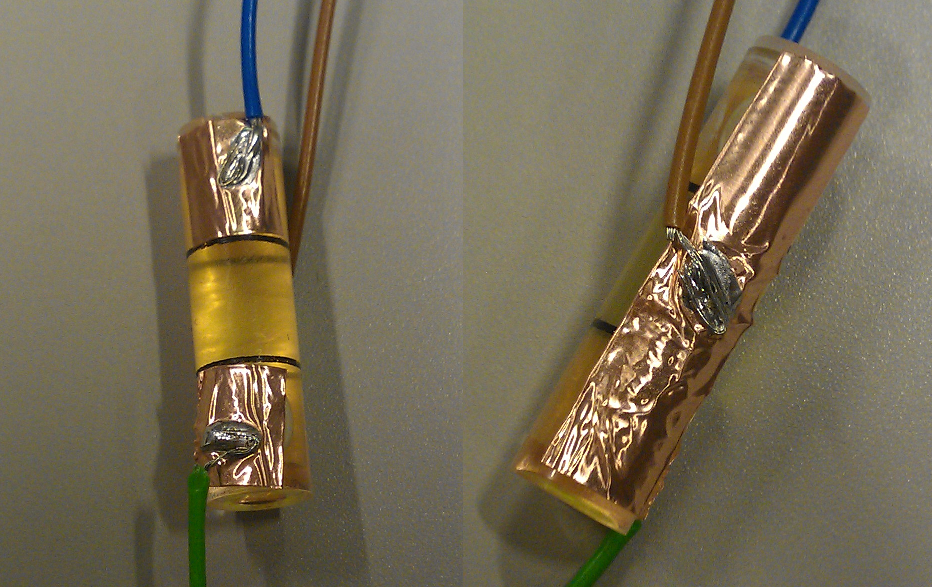
\includegraphics[width=0.5\textwidth]{billeder/libellesensor1}
\caption{henning}
\label{fig:libelle}
\end{figure}
Vi kom frem til at den har en capacitet på omkring $1*10^{-15}[F]$. Det gør det praktisk umuligt at anvende da vores filter så har en alt for stor cutoff frekvens liggende over 3.0 MHz. Den høje frekvens giver en stor selvinduktion i vores ledning. Samtidig kan vi ikke lave sinus med denne frekvens med PSoC'en. Dette gjorde at vi måtte finde en anden løsning.\\
Næste prototype bestod af et potmeter og et pendul. Dog havde potmeteret en for stor friktionsmodstand, der gjorde det upræcist i forhold til vores krav.\\
Vi har gennem et tredje semestersfag fundet ud af at PSoC'en indeholder et accelerometer. Vi valgte så at lave en prototype med det. Dette viste sig at være en god løsning.

\subsection{Metoder}
Gruppen var opsatte på at have læst review på projektets dokumentation, men de adspurgte grupper havde ingen interesse i at lave review udvekslinger. Dette har ført til at dokumentationen blev gennemlæst på et senere tidspunkt af gruppens vejleder. Grundet udskydelsen havde gruppen set sig nødsaget til at forlænge tidsplanen for at opdatere og forbedre foreløbigt færdig dokumentation. Dette førte til at design og, i sidste ende, implementering blev udskudt, hvilket medfører et stort pres imod slutningen af projektforløbet.\\
Gruppens opdeling i udviklingsmetoden har været meget flydende. Selv om der har været en projektleder og scrummaster har det ikke været nødvendigt, da gruppen har arbejdet godt sammen og diskuteret udviklingsmetoden til fuldest. Der har i forløbet været en udskiftning i koordinatorposten, hvorefter rumkoordinering har forløbet godt.\\
Gruppen har fået en bedre forståelse for eventuelt kommunikation med en kunde gennem flere iterationer af kravspecifikation.